\documentclass{article}

% Title sec
\usepackage{titlesec}

% Multicol
\usepackage{multicol}

% Figure wrapping
\usepackage{wrapfig}

% Hanging indent
\usepackage{hanging}

% color
\usepackage{xcolor}
\definecolor{LightGray}{gray}{0.9}
% APA Citation
\usepackage[
  style           = apa,
  citestyle       = authoryear,
  sorting         = nyt,
  sortcites       = true,
  autocite        = inline,
  citetracker     = false,
  maxbibnames     = 99,
  maxcitenames    = 2,
  backend         = biber,
  isbn            = false,
  doi             = true,
  urldate         = short,
  backend         = biber,
  defernumbers    = true
]{biblatex}

\DeclareBibliographyCategory{printcite}
\newcommand{\printcite}[1]{%
  \addtocategory{printcite}{#1}%
  \defbibcheck{key#1}{
    \iffieldequalstr{entrykey}{#1}
    {}
  {\skipentry}}%
  \printbibliography[heading=none,check=key#1]%
}
\addbibresource{cite.bib}

% Provide support on formatting SI Unit
\usepackage{siunitx}
\sisetup{per-mode=fraction}

% Math package
\usepackage{amsmath}
\renewcommand{\frac}{\dfrac}

\newcounter{source}
\newcommand{\sourcemeta}[3]{\subsection{Student Researcher} #1 %
  \subsection{Type} #2 %
\subsection{Citation} \printcite{#3}}

\newcommand{\source}[3]{\stepcounter{source} %
  \section{Source \#\thesource} %
\sourcemeta{#1}{#2}{#3}}

% Customized reflection entry
\newcounter{reflection}
\newcommand{\reflection}[2]{\stepcounter{reflection} %
\section*{Reflection \#\thereflection}
  %\noindent Log what you have done, what you have discovered, what you have learned, what are your next steps\ldots 

\paragraph{Date} #1

  \vspace*{-0.5cm}
\paragraph{Initials} #2}

% Customized research entry
\newcounter{research}
\newcommand{\research}[2]{\stepcounter{research} %
\section*{Source \#\theresearch}
  %\noindent Log what you have done, what you have discovered, what you have learned, what are your next steps\ldots 

\paragraph{Student Researcher} #1

  \vspace*{-0.5cm}
\paragraph{Type of Source} #2}

% Customized reference
\usepackage[hidelinks]{hyperref}

% Better typesetting
\usepackage{microtype}

% Menukeys
\usepackage[os=win]{menukeys}

% Verbatim
\usepackage{verbatim}
\usepackage{fancyvrb}
\DefineVerbatimEnvironment{MetaVerbatim}{Verbatim}{}

% Table
\usepackage{tabularx}
\usepackage{booktabs}
\usepackage{multirow}
\usepackage{makecell}
\newcolumntype{b}{>{\centering\arraybackslash}X}
\newcolumntype{s}{>{\hsize=.4\hsize\centering}X}

% Float
\usepackage{newfloat}

% 1.5 line spacing
\usepackage{setspace}
\setstretch{2.0}

% Subfigure
\usepackage{subcaption}
\usepackage{caption}

% Finer geometry
\usepackage{geometry}
\geometry{a4paper}

% Define some constants
\renewcommand{\title}{Undulatory Swimming:\\ A Topological and Computational Model}

% Define field input, i.e., box
\usepackage[most]{tcolorbox}
\newenvironment{field}{\begin{tcolorbox}[%
    enhanced, 
    breakable, 
    colback = white, colframe = black,
    sharp corners,
    boxrule = 0pt, bottomrule = 1pt, toprule = 1pt,
    leftrule = 0.5pt, rightrule = 0.5pt
]{}}{\end{tcolorbox}}

% Hanging indent
\usepackage{hanging}
\usepackage[outputdir=build]{minted} % syntax highlighting
\usepackage{longtable, booktabs}

% Enhanced list
\usepackage{enumitem}
\setitemize{noitemsep}
\setenumerate{noitemsep}

% Reset section number within part
\usepackage{chngcntr}
\counterwithin*{section}{part}

% Footer
\usepackage{fancyhdr}
\pagestyle{fancy}
\fancyhf[FR]{\hyperlink{toc}{Return to Table of Contents}}

% Glossary acronym
\usepackage[acronym]{glossaries}
\makenoidxglossaries
% dof
\newacronym{dof}{DoF}{degrees of freedom}
% ghp
\newacronym{ghp}{GHP}{Governor's Honors Program}
% rpi
\newacronym{rpi}{RPI}{Raspberry Pi}
% gpio
\newacronym{gpio}{GPIO}{General Purpose Input/Output}
% udp
\newacronym{udp}{UDP}{User Datagram Protocol}
% asr
\newacronym{asr}{ASR}{Automatic Speech Recognition}
% ml
\newacronym{ml}{ML}{Machine Learning}
% asl
\newacronym{asl}{ASL}{American Sign Language}
% gosa
\newacronym{gosa}{GOSA}{Georgia Office of Student Achievement}
% cad
\newacronym{cad}{CAD}{computer-aided design}
% sd
\newacronym{sd}{SD}{speaker diarization}
% vad
\newacronym{vad}{VAD}{voice activation detection}
% stt
\newacronym{stt}{STT}{speech-to-text}
% mvp
\newacronym{mvp}{MVP}{minimum viable product}
% cs
\newacronym{cs}{CS}{computer science}
% Table of contents title change
\renewcommand{\contentsname}{Table of Contents}

% Part and Subpart only
\setcounter{tocdepth}{-1}

\begin{document}
\begin{titlepage}
  \centering
  \vspace*{1in}
  \begin{tikzpicture}[overlay,remember picture]
    \node[anchor=center, opacity=0.15, xshift=2cm, yshift=2cm] at (current page.center) {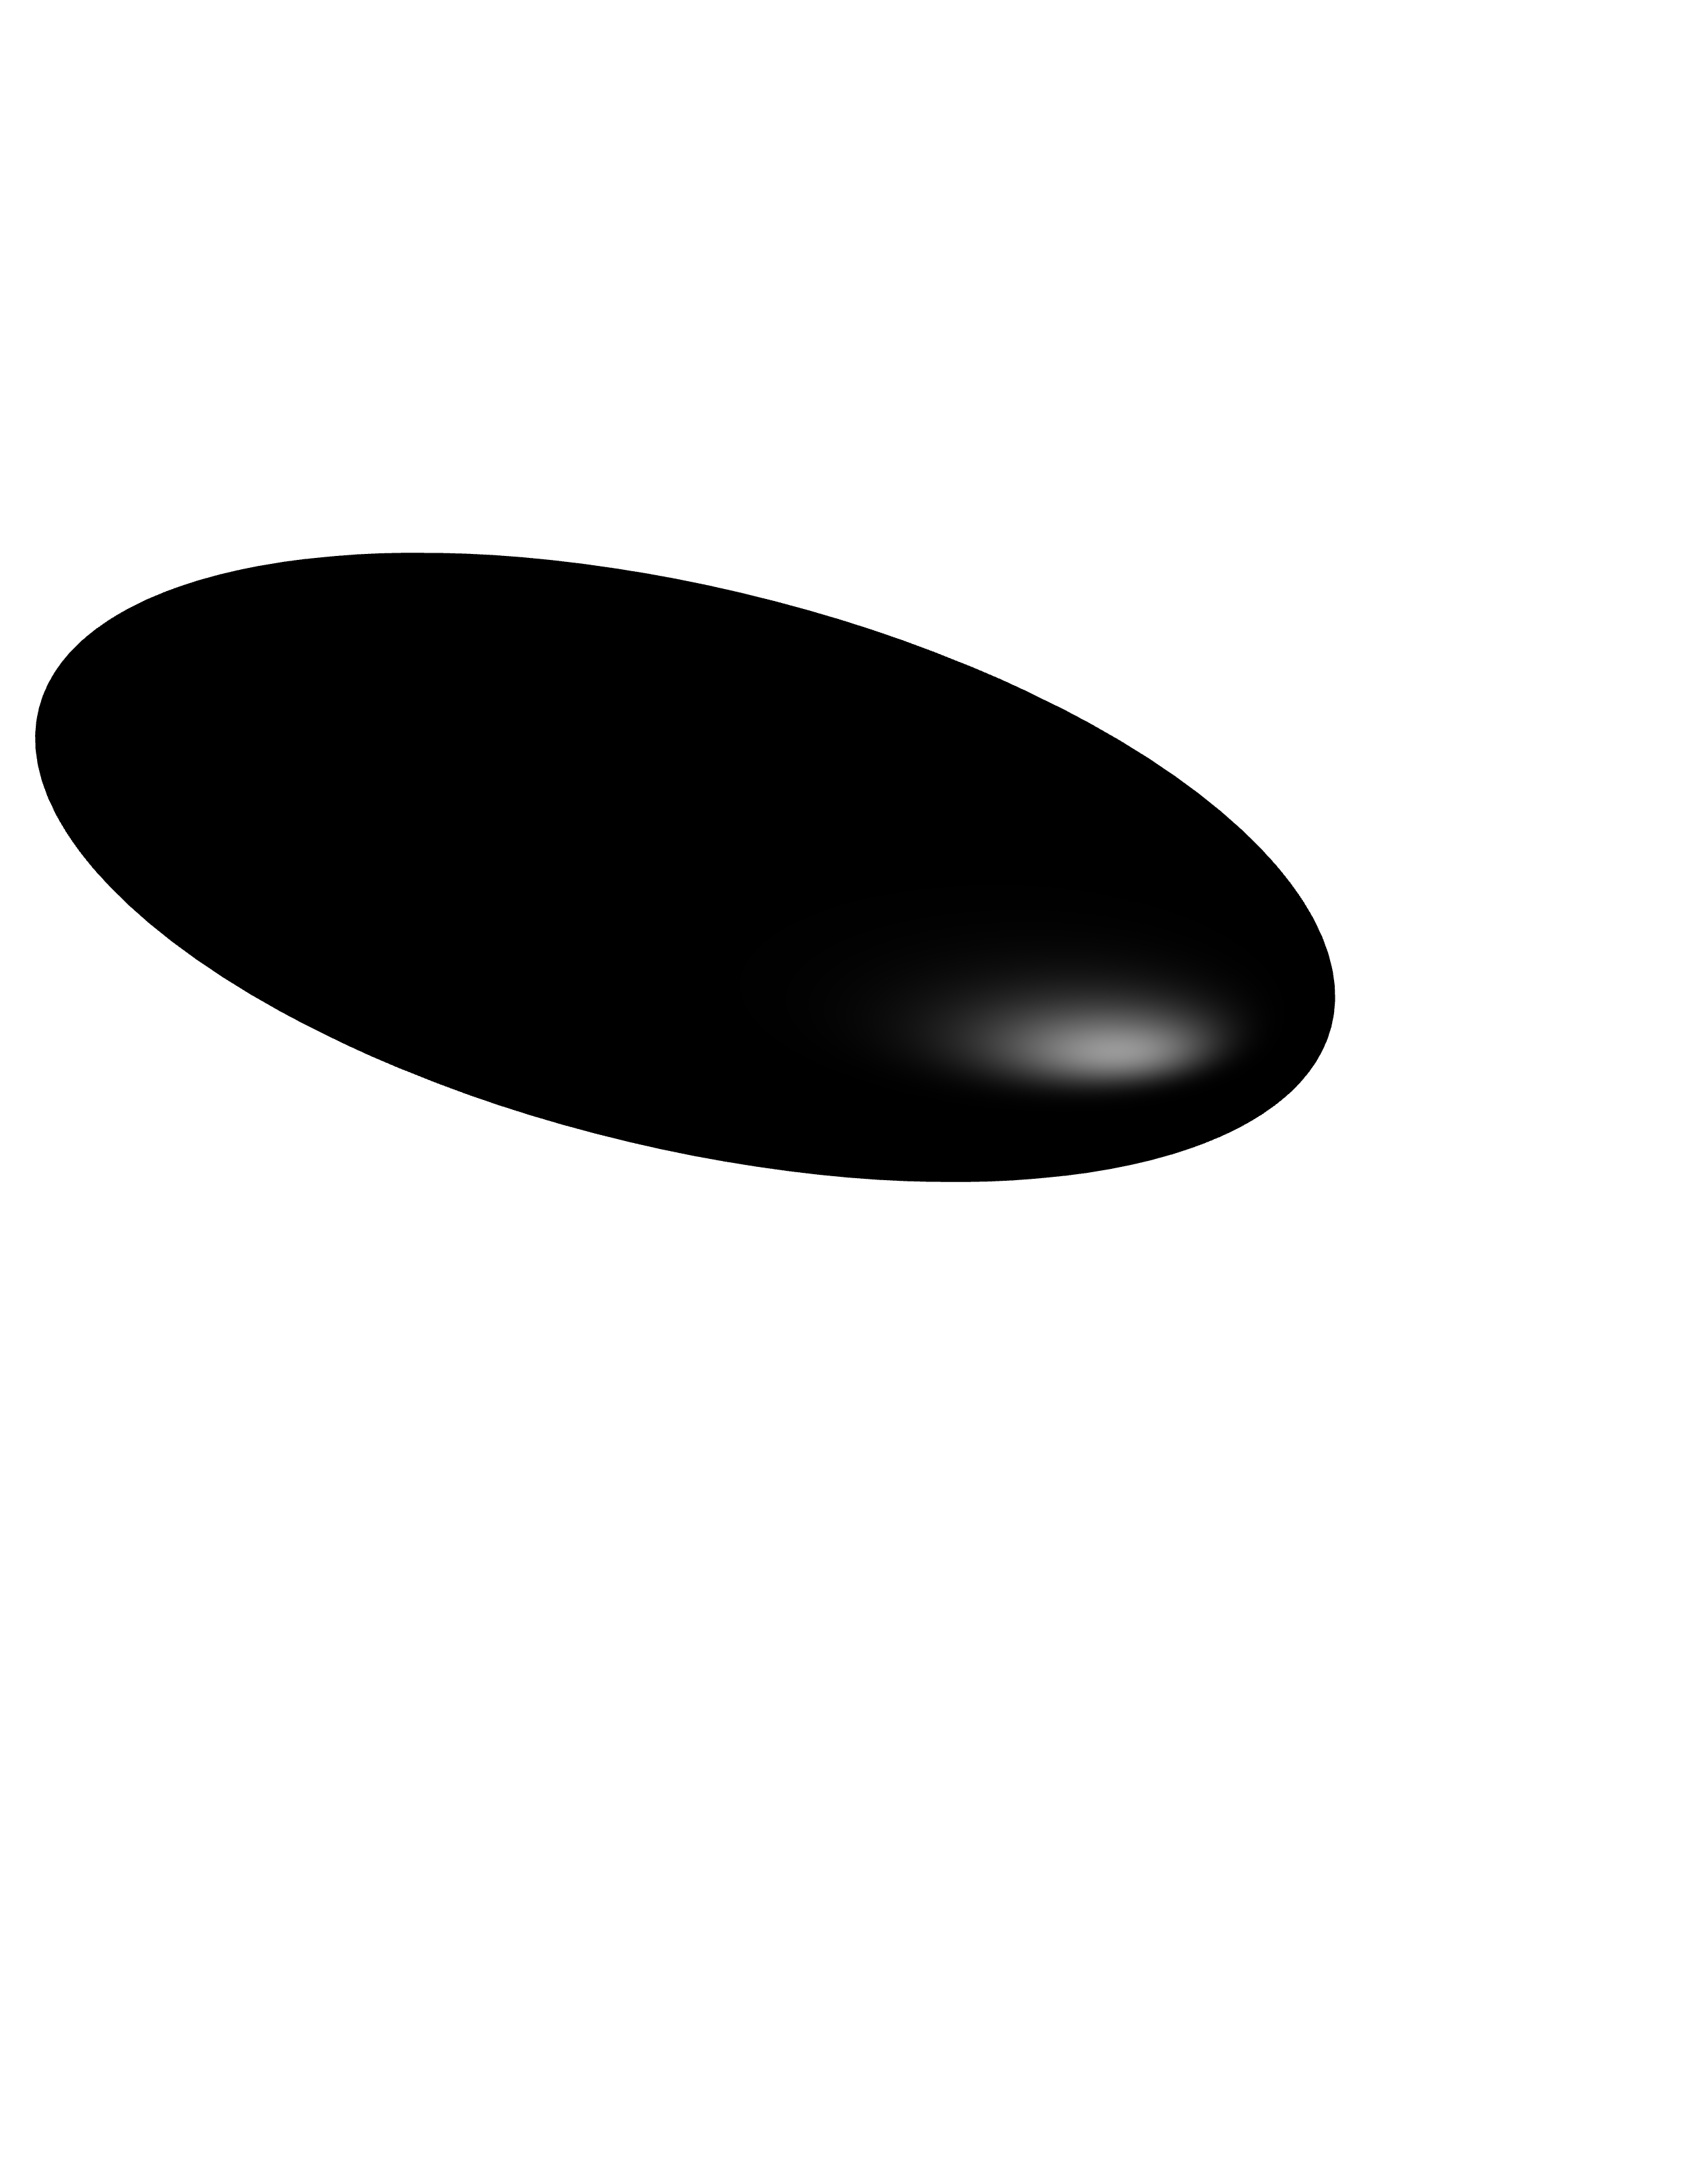
\includegraphics[width=\paperwidth]{media/cad.png}};
  \end{tikzpicture}
  {\fontsize{56pt}{2\baselineskip}\selectfont \bfseries
  \title}
  \vfill

  \Large
  Gwinnett School of Math, Science, and Technology\\
  Lawrenceville, Georgia

  \vspace{0.5in}
  \setstretch{1.15}\selectfont

  \vspace{1em}
  \textbf{Team Leader}\\ Dobromir Iliev

  \vspace{1em}
  \textbf{Team Members}\\ Anish Goyal \& Ricardo Guardado

  \vspace{1em}
  \textbf{12 April 2024}
\end{titlepage}
\tableofcontents
\newpage

%\part{Directions and Tips}

Delete this entire page before submitting FINAL logbook check (not before)

\begin{itemize}
    \item Remember that this is a legal document.
    \item Anyone should be able to follow exactly what you did in your project
          by reading your logbook. That's the level of detail you need.
    \item You MAY NOT delete any entries/data from this notebook. If you need to
          delete anything, you should strike through it (\menu{format > text >
          strikethrough}). You can also make multiple versions of your entries,
          if appropriate.
    \item If you did work on other documents, you may cut and paste the items
          from those other locations. Just provide citations/reference those
          other locations. If you can't cut \& paste easily (like you are
          referencing a physical lab notebook), you should decide if it's
          important to scan in the document or to just reference your previous
          work.
\end{itemize}

EVERY SKETCH OR DESIGN OR CODE you create should be included in your journal.
Every design change must be documented. If you have any physical lab set ups or
things you are building, include photos in your reflection entries. You must
have AT LEAST SOME PICTURES that include you doing work on your project.

\begin{itemize}
    \item Every day you work on a project, you should include a reflection entry
          with a summary of what you accomplished that day, any ideas you
          discussed, and other important ideas (even if you're not sure and are
          just considering them).
    \item Use your reflection entries to plan out what your next day should
          accomplish.
    \item At some point, you will need to do project planning, and you should
          include images of your project planning document (like a kanban board
          in your journal).
    \item Research/bibliography pages should be set up correctly using proper.
    \item If appropriate, title your entries (not reflection entries but other
          items in your lab notebook). You can insert ADDITIONAL sections in
          your logbook, but you must have everything in the template.
    \item Date all entries and put your initials. If you modify the entry, put
          modified dates and re-initial. You can also make version 1, 2, etc.\@
          for entries. Include page numbers
\end{itemize}

\part{Brainstorming}

\begin{itemize}
    \item Enhanced Biomimicry: investigate other organisms with unique undulatory swimming patterns and incorporate those patterns into our design.
    \item Explore aspects of fish locomotion, such as lateral line sensing, and integrate them for improved efficiency.
    \item Advanced Fluid Dynamics Modeling: Refine the computational fluid dynamics (CFD) model by incorporating real-time environmental data, allowing for dynamic adjustments in response to changing conditions.
    \item Turbulence and water currents in the CFD model to simulate more realistic aquatic environments.
    \item Machine Learning Integration: Implement machine learning algorithms to optimize the undulatory swimming patterns based on real-time feedback from the environment.
    \item Train the system to adapt to different terrains, depths, or obstacles for enhanced autonomy.
    \item Sustainable Materials: exploring sustainable materials research for 3D printing the model, aligning with ecological considerations for underwater exploration.
    \item Multi-Agent Systems, investigating the feasibility of deploying multiple submersibles working collaboratively in a swarm, sharing information and optimizing propulsion collectively.
    \item Sensory integration, by integrating additional sensors, such as temperature or pressure sensors, to expand the submersible's data collection capabilities and environmental awareness.
    \item Energy harvesting which is the implementation of energy harvesting technologies, such as solar or hydrodynamic energy, to supplement the power source and extend the operational duration.
    \item Adaptive control strategies: Develop adaptive control strategies that allow the submersible to dynamically adjust its undulatory motion based on real-time sensory input, optimizing energy efficiency.
    \item Underwater communication: enhance communication capabilities for remote operation, possibly through acoustic or optical communication methods.
    \item Underwater Navigation and Mapping: Incorporate navigation algorithms to enable the submersible to autonomously navigate and map underwater environments, contributing to ocean exploration.
    \item Integration with Environmental Monitoring: Explore possibilities for integrating environmental sensors that contribute to scientific data collection, such as monitoring water quality, temperature, or marine life.
    \item Humanitarian and Environmental Applications: Explore applications in environmental conservation, such as monitoring coral reefs or underwater ecosystems, contributing to biodiversity preservation.
    \item Collaboration with Marine Biologists: Collaborate with marine biologists to gain insights into specific fish behaviors and optimize the submersible's design accordingly.
    \item Educational Outreach: Develop educational materials and outreach programs to engage students and the public in understanding the importance of biomimicry and robotics in ocean exploration.
    \item Miniaturization and Micro-Robotics: Investigate the feasibility of miniaturizing the design for applications in confined underwater spaces or for studying microorganisms.    
\end{itemize}
\addtocontents{toc}{\protect\hypertarget{toc}{}}
\part{Research}
\source{<student contributor name>}{<source type>}{<biblatex citation>}

\subsection{Note}

\subsection{Implication}
\newpage

\part{Reflections}
\reflection{<date>}{<reflector name>}


\newpage

\part{Required Forms}

\textbf{The required forms for this project are:}

\begin{itemize}
  \item GSEF Participation Agreement
  \item Official GSEF Abstract Form
  \item Checklist for Adult Sponsor [Form 1]
  \item Checklist for Adult Sponsor [Form 1a]
  \item Research Plan/Project Summary
  \item Approval [Form 1B]
\end{itemize}

\textbf{They can be found on the following pages.}

\part{Research Plan}
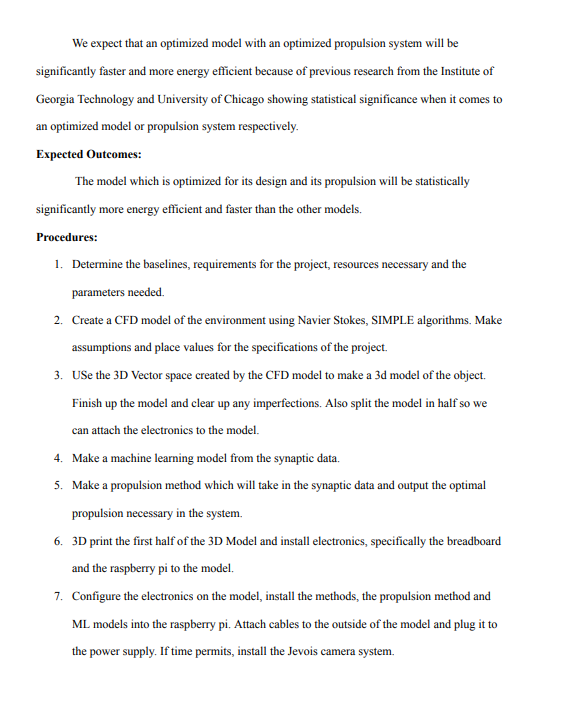
\includegraphics[width=\textwidth]{media/image6}
\newpage
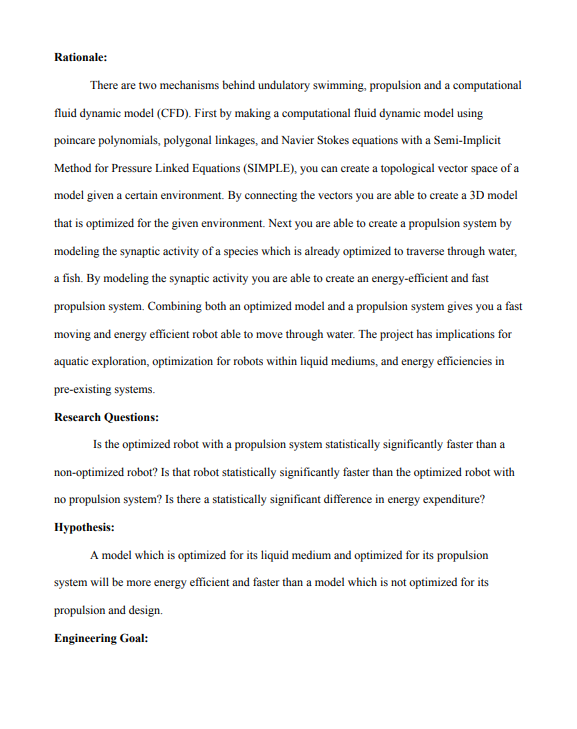
\includegraphics[width=\textwidth]{media/image9}
\newpage
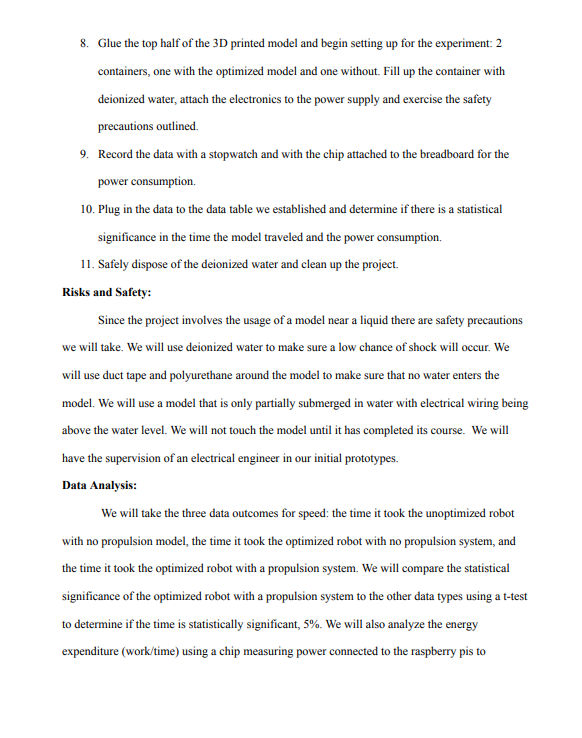
\includegraphics[width=\textwidth]{media/image10}
\newpage
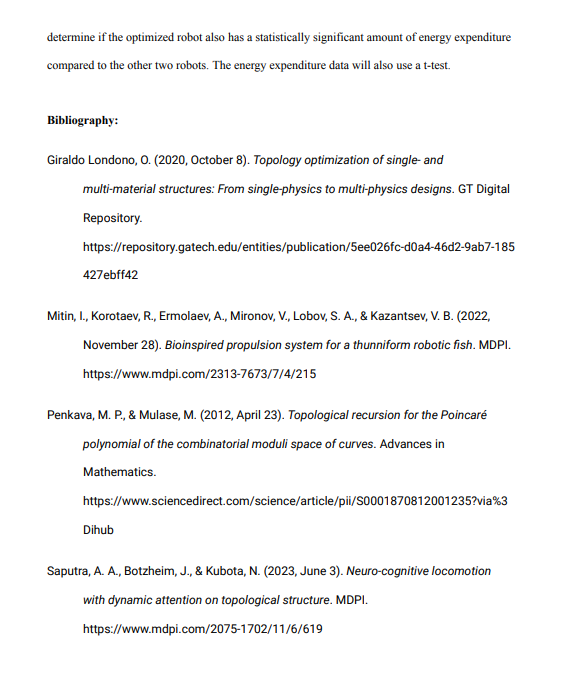
\includegraphics[width=\textwidth]{media/image28}

\part{Risk Assessment Form}
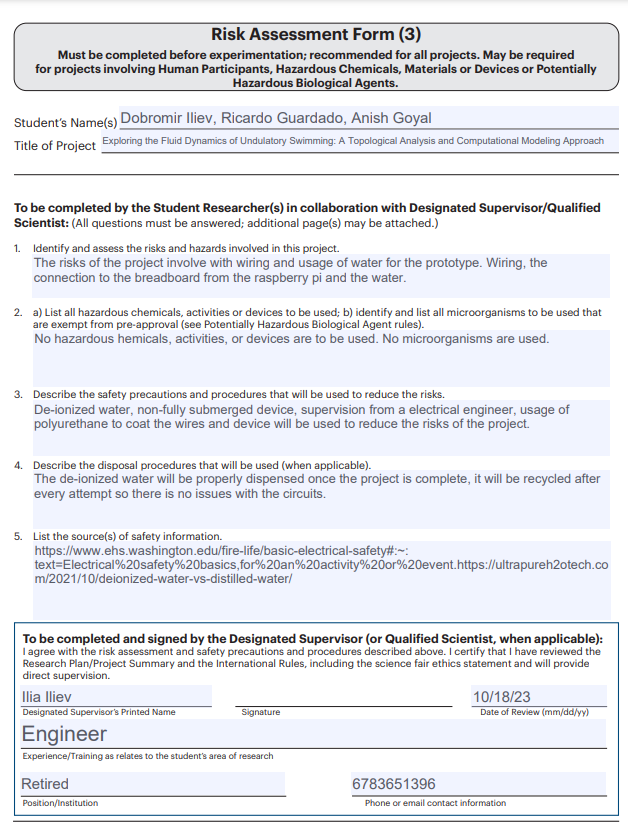
\includegraphics[width=\textwidth, height=1.2\textwidth]{media/image17.png}

\newpage

\part{Student Checklist}
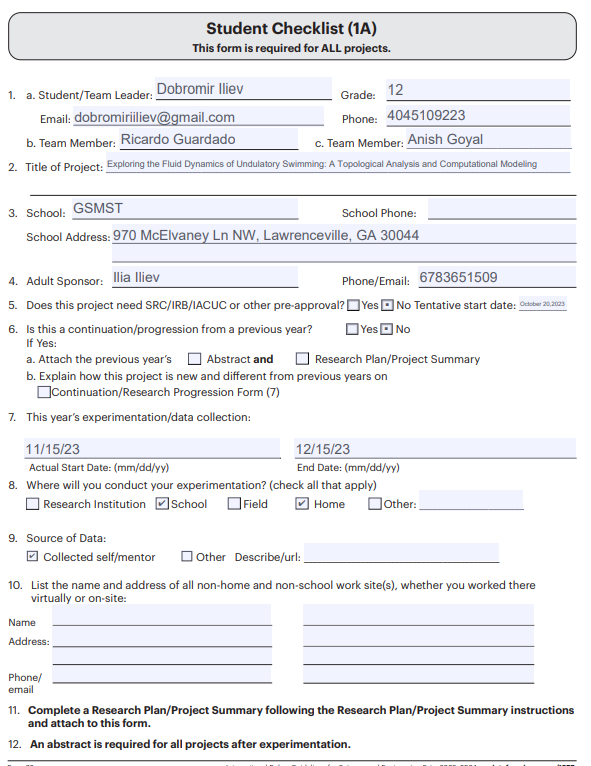
\includegraphics[width=\textwidth]{media/image41.png}

\newpage

\part{Research Question/Goal}

\textbf{What are you trying to accomplish?}

The rationale for the project is that by incorporating models for synaptic activity and a model you can create a more energy efficient system. Zebrafish are meant to be in homeostasis, therefore biomimicry based upon their movement is likely to be more energy efficient. Additionally pre existing research showcases how the computational fluid dynamic model is efficient in solid state structures, therefore, there is precedent in the model working for a robotic model in aquatics. The unique challenges and conditions of the ocean can be represented with  the model.

\newpage 

\part{Hypothesis}

\textbf{Include your independent and dependent variables AND justification for your hypothesis. Engineering projects also need a hypothesis because they must test their concepts. Include a separate null hypothesis.}

Experimental hypothesis: The biomimetic propulsion system and topological model will exhibit statistically significant differences in energy expenditure.

Null Hypothesis: The biomimetic propulsion system and topological model does not differ in efficiency compared to the traditional propulsion system.

\newpage

\part{Data}
\newpage

\part{Graphs}
\newpage

\part{Statistical Analysis}
\newpage

\part{Photo Documentation}
\newpage

% print bibliography
\nocite{*}
\printbibliography

\end{document} 